\documentclass[tikz]{standalone}
\usepackage[blue]{causets}
\usetikzlibrary{fit,shapes.geometric}
\begin{document}
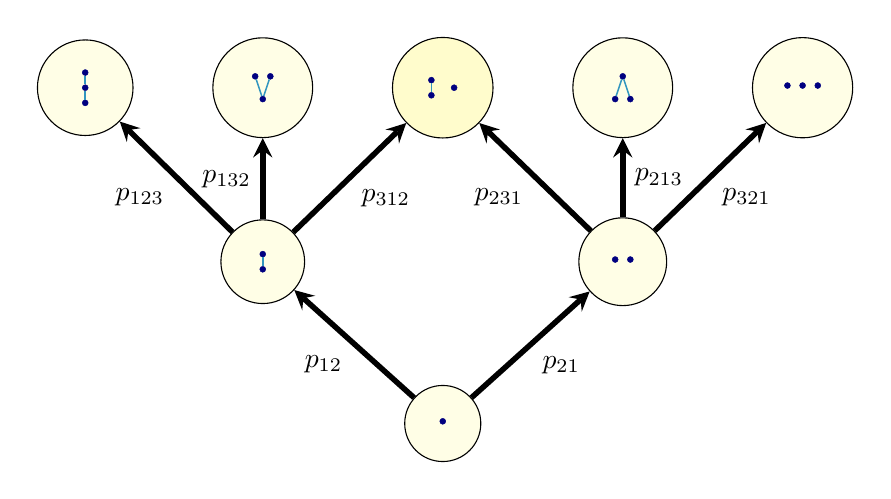
\begin{tikzpicture}[-stealth, line width=2pt]
	\matrix[nodes={draw, fill=yellow!10, thin, circle, inner sep=1.7ex}, row sep=1cm, column sep=1cm]
	{
		\node (C123) {\pcauset{1,2,3}}; 
	& \node (C132) {\pcauset{1,3,2}}; 
	& \node[fill=yellow!20] (C312) {\pcauset{3,1,2}}; 
	& \node (C213) {\pcauset{2,1,3}}; 
	& \node (C321) {\pcauset{3,2,1}}; 
	\\
	& \node (C12) {\pcauset{1,2}}; 
	& 
	& \node (C21) {\pcauset{2,1}}; 
	\\
	& 
	& \node (C1) {\pcauset{1}}; 
	\\
	};
	\draw (C1) -- node[below left] {$p_{12}$} (C12);
	\draw (C12) -- node[below left] {$p_{123}$} (C123);
	\draw (C12) -- node[left] {$p_{132}$} (C132);
	\draw (C12) -- node[below right] {$p_{312}$} (C312);
	\draw (C1) -- node[below right] {$p_{21}$} (C21);
	\draw (C21) -- node[below left] {$p_{231}$} (C312);
	\draw (C21) -- node[right] {$p_{213}$} (C213);
	\draw (C21) -- node[below right] {$p_{321}$} (C321);
\end{tikzpicture}
\end{document}
